
\usepackage{fancyhdr}
\usepackage{lastpage}
\usepackage[utf8]{inputenc}

% Minted for syntax highliting
\usepackage{minted}
\usemintedstyle{tango}

% 
\usepackage[T1]{fontenc}
\usepackage{lmodern}

\usepackage{calc}
\usepackage{bytefield}

\usepackage{listings}
\usepackage{amsmath}

\usepackage{tikz}
\usetikzlibrary{automata,arrows,topaths,calc,positioning}
 
\usepackage{syntax}
\grammarindent=2cm


% Headers/footers styling
\pagestyle{fancy}
\fancyhf{}
\renewcommand{\headrulewidth}{0pt}

% Footer
\lfoot{ID1019}
\cfoot{KTH}
\rfoot{\thepage \hspace{1pt} / \pageref{LastPage}}

%\newcommand{\defaultpagestyle}{\thispagestyle{plain}}
\newcommand{\defaultpagestyle}{\thispagestyle{fancy}}



\title[ID1019 Data structures]{Data structures}


\author{Johan Montelius}
\institute{KTH}
\date{\semester}

\begin{document}

\begin{frame}
\titlepage
\end{frame}

\begin{frame}{first a recap}

\pause In functional programming, a program is a set of functions.

\vspace{20pt}\pause A function takes some arguments and {\em returns a result} \ldots it does not change the given arguments.

\vspace{20pt}\pause The returned value of a function is only depending on the given arguments.

\vspace{20pt}\pause Fundamentally different from {\em imperative programming}!


\end{frame}


\begin{frame}{Data structures}

  \begin{itemize}
  \item integers, floting point values \pause
  \item boolean - true or false
  \item atoms - similar to Java enum \pause
  \item tuples - similar to a C struct but without names or an array\pause
  \item lists - syntax for linked lists
  \item strings, chars, char-lists - "hello", ?h, ?e, ?l, ?l, ?o, 'hello'
  \end{itemize}

\end{frame}

\begin{frame}{Integers}

  Syntax:
  \space{10pt}
  \begin{itemize}
  \item 12345 \pause
  \item 0b1010101 \pause
  \item 0x1F \pause
  \end{itemize}  
  
  Integgers can be almost arbitrary large: \pause

  \vspace{10pt}\
  {\tt > 123456789123456789 * 123456789123456789}\pause

  {\tt 15241578780673678515622620750190521} \pause
  
  \vspace{20pt}\pause
  {\em arithmetic could be slow}
\end{frame}

\begin{frame}{Floating points}

  Syntax:
  \space{10pt}
  \begin{itemize}
  \item 1.2345 \pause
  \item 1.2345E6 \pause
  \end{itemize}

  \space{20pt}
  {\tt 2.0 == 2} is true  but {\tt 2.0 === 2} is not true

  \vspace{20pt}\pause
  {\em arithmetic is slow}  
\end{frame}

\begin{frame}{atoms}

  Atoms are identifiers with a program whide scope. \pause

  \vspace{20pt}
  Used to represent objects or values : {\tt :apple}, {\tt :orange}, {\tt :ok}, {\tt :error}. \pause

  \vspace{20pt}
  The atoms {\tt :true} and {\tt :false} are used to represent boolan {\em true} and {\em false}.\pause
  

  \vspace{20pt}
  {\em syntax allows to ommit colon fo the atoms {\tt :true}, {\tt :false} and {\tt :nil}.}
    
\end{frame}

\begin{frame}[fragile]{module names}

  \begin{lstlisting}
    defmodule Foo do

      def bar(x) do
         br = Bar.answer(x)
         :io.format("FooBar = ~w\n", [br])
      end

    end
  \end{lstlisting}

  \vspace{20pt}
  {\em {\tt Foo} is an alias for an atom {\tt :"Elixir.Foo"}.}
  
\end{frame}


\begin{frame}[fragile]{dynamic typing}

  No type declaration in code.

  \begin{columns}
   \begin{column}{0.5\textwidth}
    \begin{lstlisting}
def test(x, y) do
  if (x == 0) do
    y
  else 
    x + y
  end
end
     \end{lstlisting}
   \end{column}
   \begin{column}{0.5\textwidth}
    \begin{lstlisting}
def Int test(Int x, Int y) do
  if (x == 0) do
    y
  else 
    x + y
  end
end
     \end{lstlisting}
   \end{column}   
 \end{columns}


 \vspace{20pt}
{\em types are checked at runtime}
 
\end{frame}


\begin{frame}{tuples}

  A compund data structure. \pause

  \vspace{20pt}

  {\tt \{:orange, 23, "Goda appelsiner från Spanien"\}}  \pause

  \vspace{20pt}

  {\em You need to keep track or the order: type, price, sales pitch.}

\end{frame}

\begin{frame}[fragile]{tuples}

  No declarations of tuples but we have a language to describe them
  for documentation.\pause

  \vspace{20pt}  
  \begin{lstlisting}
@type name() :: :orange | :tomato | :cucumber

@type product() :: {name(), integer(), string()}
  \end{lstlisting}

  \pause
  \vspace{10pt}
  {\em more on this later}

\end{frame}

\begin{frame}[fragile]{access components}

  Components of a tuple are extarcted using {\em pattern matching}.\pause

  \begin{lstlisting}
    x = {:gurka, 123, "Prima gurkor"}
  \end{lstlisting}

  \pause
  \vspace{20pt}

  \begin{lstlisting}
    {type, price, _} = x 
  \end{lstlisting}  

  \vspace{20pt}

  \begin{lstlisting}
    price = elem(x, 1)   # zero indexed!
  \end{lstlisting}    

  \vspace{10pt}
  {\em If you use {\tt elem}, you most likely don't know how to use pattern matching.}
  
\end{frame}

\begin{frame}{under the hood}

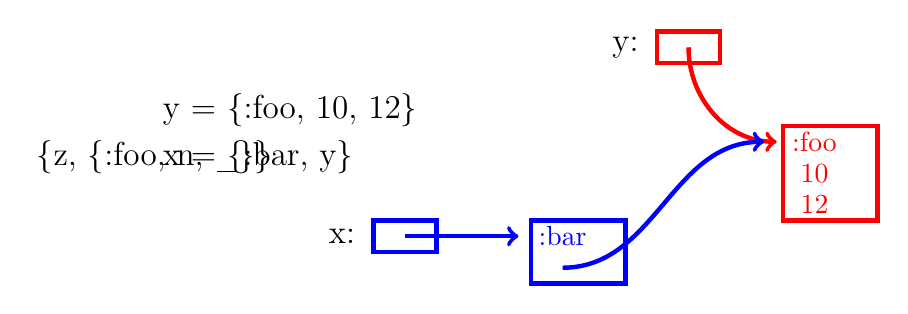
\begin{tikzpicture}[scale=0.4]


\node[anchor=west] at (0,6.5) {{\large y = \{:foo, 10, 12\}}};

\node at (15,8.5) {{\large y:}};
\draw[ultra thick, red] (16,8) rectangle +(2,1);
\draw[ultra thick, red] (20,6)rectangle +(3,-3);
\node[ultra thick, red] at (21,5.5) {:foo};
\node[ultra thick, red] at (21,4.5) {10};
\node[ultra thick, red] at (21,3.5) {12};
\draw[ultra thick, red, ->] (17,8.5) to[out=270,in=180]  (19.8,5.5);

\pause 
\node[anchor=west] at (0,5) {{\large x = \{:bar, y\}}};
\pause 
\node at (6,2.5) {{\large x:}};
\draw [ultra thick, blue] (7,2) rectangle +(2,1);
\draw[ultra thick, blue] (12,3)rectangle +(3,-2);
\node[ultra thick, blue] at (13,2.5) {:bar};
\draw[ultra thick, blue, ->] (13,1.5) to[out=0,in=180]  (19.4,5.5);
\draw[ultra thick, blue, ->] (8,2.5) to[out=0,in=180]  (11.6,2.5);

\pause
\node[anchor=west] at (-4,5) {{\large \{z, \{:foo, n, _\}\}}};

\end{tikzpicture}

\end{frame}



\begin{frame}[fragile]{linked list}

  In functional programming languages linked lista are very useful.\pause

  \vspace{20pt}
  \begin{lstlisting}
    []
  \end{lstlisting}
  \vspace{10pt}\pause
  \begin{lstlisting}
    [:one, 2, "three", 4]
  \end{lstlisting}  
  
\end{frame}

\begin{frame}[fragile]{the cons operator}

  Creating a new node:\pause

  \vspace{20pt}
  \begin{lstlisting}
    foo = 1
    rest = [2,3,4,5]
    all = [ foo | rest] 
  \end{lstlisting}
  \vspace{10pt}\pause
  \begin{lstlisting}
    [1,2,3,4,5]
  \end{lstlisting}  
  
\end{frame}

\begin{frame}[fragile]{list patterns}

  \vspace{20pt}
  \begin{lstlisting}
    [a, b, c] = [1,2,3]
  \end{lstlisting}
  \vspace{10pt}\pause
  \begin{lstlisting}
    [a | rest] = [1,2,3]
  \end{lstlisting}  

  \vspace{10pt}\pause
  \begin{lstlisting}
    [a, b | rest] = [1,2,3]
  \end{lstlisting}    

  \vspace{10pt}\pause
  \begin{lstlisting}
    [a | rest] = [1]
  \end{lstlisting}    
\end{frame}


\begin{frame}{exercise}
\begin{itemize}
\pause \item  {\tt [h|t] = [:a,[:b,:c]]}  
\pause \item  {\tt [h1,h2|t] = [:a,:b,:c]} 
\pause \item  {\tt [h1,h2,t] = [:a,:b,:c]} 
\pause \item  {\tt [h1,h2,t] = [:a,:b,:c,:d]} 
\pause \item  {\tt [h1|[h2|t]] = [:a,:b,:c]}
\pause \item  {\tt [h|t] = [:a|:b]}
\end{itemize}
\end{frame}

\begin{frame}{list construction}
\begin{itemize}
\pause \item  {\tt h = :a; t = [:b]; [h|t]}
\pause \item  {\tt h = :a; t = [[:b]]; [h|t]}
\pause \item  {\tt h = [:a,:b]; t = [:c,:d]; [h|t]}
\pause \item  {\tt h = [:a,:b]; t = [:c,:d]; [h,t]}
\pause \item  {\tt h1 = [:a,:b]; h2 = [:c,:d]; t = [:e,:f]; [h1|[h2|t]]}
\pause \item  {\tt h1 = [:a,:b]; h2 = [:c,:d]; t = [:e,:f]; [h1,[h2|t]]}
\pause \item  {\tt h = [:a,:b]; t = :c; [h|t]}
\end{itemize}
\end{frame}


\begin{frame}{cons cells}

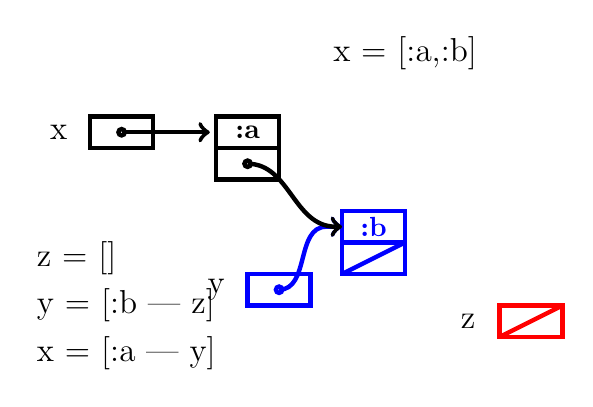
\begin{tikzpicture}[scale=0.4]

\node[anchor=west] at (0,3.5) {{\large z = []}};

\node at (14,1.5) {{\large z}};
\draw [ultra thick, red] (15,1) rectangle +(2,1);
\draw [ultra thick, red] (15,1) -- +(2,1);

\pause 
\node[anchor=west] at (0,2) {{\large y = [:b | z]}};
\pause 
\node at (6,2.5) {{\large y }};
\draw [ultra thick, blue] (7,2) rectangle +(2,1);
\pause 
\draw [ultra thick, blue] (10,4) rectangle +(2,1) node at +(1,0.5) {{\bf :b}};
\draw [ultra thick, blue] (10,3) rectangle +(2,1);
\draw [ultra thick, blue] (10,3) -- +(2,1);
\pause 
\draw [ultra thick, blue] (8, 2.5) circle [radius =0.1];
\draw [ultra thick, blue] (8,2.5)  to [out=0, in=180]  (9.5,4.5);
\draw [ultra thick, blue, ->] (9.5,4.5) -- (10,4.5); 

\pause 
\node[anchor=west] at (0,0.5) {{\large x = [:a | y]}};
\pause 
\node at (1,7.5) {{\large x }};
\draw [ultra thick, black] (2,7) rectangle +(2,1);
\pause 
\draw [ultra thick, black] (6,7) rectangle +(2,1) node at +(1,0.5) {{\bf :a}};
\draw [ultra thick, black] (6,6)  rectangle +(2,1);
\pause 

\draw [ultra thick, black] (7, 6.5) circle [radius =0.1];
\draw [ultra thick, black] (7,6.5)  to [out=0, in=180]  (9.8,4.5);
\draw [ultra thick, black, ->] (9.8, 4.5) -- (10,4.5);
\pause 
\draw [ultra thick, black] (3, 7.5) circle [radius =0.1];
\draw [ultra thick, black, ->] (3,7.5) -- (5.8, 7.5); 
\pause
\node at (12,10) {{\large x = [:a,:b] }};

\end{tikzpicture}

\end{frame}


\begin{frame}[fragile]{Strings}

\begin{verbatim}
text = "This is a string"
\end{verbatim}
  
\vspace{20pt}  \pause
  
\begin{verbatim}
combined = text <> " that we append to this string"
\end{verbatim}

\vspace{20pt}  \pause

\begin{verbatim}
answer = 42
message = "The answer is #{answer}, but what is question?"
\end{verbatim}

\end{frame}

\begin{frame}[fragile]{Strings and binaries}

\vspace{20pt}  \pause
\begin{verbatim}  
  <<x, y, z , rest::binary>> = "absdefg"
\end{verbatim}  
  
\end{frame}

\begin{frame}[fragile]{Strings and lists of charactes}

\vspace{20pt}  \pause  
\begin{verbatim}
  msg = String.to_charlist("abcde")
\end{verbatim}

\vspace{20pt}  \pause
\begin{verbatim}  
  [x,y,z | rest] = msg
\end{verbatim}

\vspace{20pt}  \pause
\begin{verbatim}  
  msg = [?h, ?e, ?l, ?l, ?o]
\end{verbatim}

\end{frame}

\begin{frame}{Summary}

  \begin{itemize}
  \item integers, floting point values \pause
  \item boolean - true or false
  \item atoms - similar to Java enum \pause
  \item tuples - similar to a C struct (but without names) or an array\pause
  \item lists - syntax for linked lists
  \item strings, chars, char-lists  - "hello", ?h, ?e, ?l, ?l, ?o, 'hello'
  \end{itemize}

\end{frame}

\end{document}


